\documentclass[10pt]{article}\usepackage[]{graphicx}\usepackage[]{color}
%% maxwidth is the original width if it is less than linewidth
%% otherwise use linewidth (to make sure the graphics do not exceed the margin)
\makeatletter
\def\maxwidth{ %
  \ifdim\Gin@nat@width>\linewidth
    \linewidth
  \else
    \Gin@nat@width
  \fi
}
\makeatother

\definecolor{fgcolor}{rgb}{0.345, 0.345, 0.345}
\newcommand{\hlnum}[1]{\textcolor[rgb]{0.686,0.059,0.569}{#1}}%
\newcommand{\hlstr}[1]{\textcolor[rgb]{0.192,0.494,0.8}{#1}}%
\newcommand{\hlcom}[1]{\textcolor[rgb]{0.678,0.584,0.686}{\textit{#1}}}%
\newcommand{\hlopt}[1]{\textcolor[rgb]{0,0,0}{#1}}%
\newcommand{\hlstd}[1]{\textcolor[rgb]{0.345,0.345,0.345}{#1}}%
\newcommand{\hlkwa}[1]{\textcolor[rgb]{0.161,0.373,0.58}{\textbf{#1}}}%
\newcommand{\hlkwb}[1]{\textcolor[rgb]{0.69,0.353,0.396}{#1}}%
\newcommand{\hlkwc}[1]{\textcolor[rgb]{0.333,0.667,0.333}{#1}}%
\newcommand{\hlkwd}[1]{\textcolor[rgb]{0.737,0.353,0.396}{\textbf{#1}}}%

\usepackage{framed}
\makeatletter
\newenvironment{kframe}{%
 \def\at@end@of@kframe{}%
 \ifinner\ifhmode%
  \def\at@end@of@kframe{\end{minipage}}%
  \begin{minipage}{\columnwidth}%
 \fi\fi%
 \def\FrameCommand##1{\hskip\@totalleftmargin \hskip-\fboxsep
 \colorbox{shadecolor}{##1}\hskip-\fboxsep
     % There is no \\@totalrightmargin, so:
     \hskip-\linewidth \hskip-\@totalleftmargin \hskip\columnwidth}%
 \MakeFramed {\advance\hsize-\width
   \@totalleftmargin\z@ \linewidth\hsize
   \@setminipage}}%
 {\par\unskip\endMakeFramed%
 \at@end@of@kframe}
\makeatother

\definecolor{shadecolor}{rgb}{.97, .97, .97}
\definecolor{messagecolor}{rgb}{0, 0, 0}
\definecolor{warningcolor}{rgb}{1, 0, 1}
\definecolor{errorcolor}{rgb}{1, 0, 0}
\newenvironment{knitrout}{}{} % an empty environment to be redefined in TeX

\usepackage{alltt}
\usepackage[utf8]{inputenc}
\usepackage[spanish,activeacute]{babel}
\usepackage{amsmath}
\usepackage{amsfonts}
\usepackage{amssymb}
\usepackage{graphicx}
\usepackage{vmargin}
\usepackage{listings}
\usepackage{listings}						% Para el código Fuente


\setpapersize{A4}
\setmargins{2cm}       % margen izquierdo
{1cm}                        % margen superior
{16.5cm}                      % anchura del texto
{23.42cm}                    % altura del texto
{10pt}                           % altura de los encabezados
{1cm}                           % espacio entre el texto y los encabezados
{0pt}                             % altura del pie de p�gina
{2cm}                           % espacio entre el texto y el pie de p�gina
\IfFileExists{upquote.sty}{\usepackage{upquote}}{}
\begin{document}
	
\begin{center}
	{\Large \textbf{Programaci\'{o}n de Aplicaciones para Internet y la Nube  \hspace{1cm}	2016-I}}\\
\end{center}

	\begin{flushright}
		{\large \textbf{Informe de lectura: Dynamic Documents with R and knitr : Cross Reference\\
		``Documentos Dinámicos con R y knitr: Referencias Cruzadas"}}
		
	\end{flushright}
	\textbf{Wilson Ricardo L'opez S'anchez\\	
	Fecha de evaluaci'on 1 de abril del 2016\\}\\
\\


  \textbf{Resumen:}
\\	
	
	El capítulo de referencias cruzadas habla sobre la utilización de códigos de R a través de un documento externo como es el caso de html, latex entre otros, por medio de paquete de R llamada Knitr, entre las ventajas que nos ofrece las referencias cruzadas están:
	
	\begin{itemize}
		
		
	
\item	la utilización de código a través de todo el documento, ejecutándolo y mostrando los resultados en el mismo 

\item	reutilización de diferentes códigos a través de todo el documento.

\item	Utilización de códigos dentro de otros códigos por medio de etiquetas

\item	También es posible llamar códigos guardados que se encuentran dentro de la misma carpeta del documento principal.

\item	La asignación de diferentes etiquetas a diferentes partes de un código que se encuentra guardado, para ser utilizadas a lo largo de todo el código.

\item	La utilización de un documento principal y de códigos hijos para así tener una mejor organización del documento principal 

\item	La utilización del encabezado del documento principal para compilar códigos que ni tienen encabezado o códigos que no fueron desarrollados para el documento principal si no que son totalmente apartes.

\end{itemize}
Para la demostración y utilización de las características mencionadas anteriormente se utilizará Rstudio tanto para la compilación de código R y del documento latex. 
\\
\\
	
\newpage

\textbf{Contribución al desarrollo de la programación literaria: Referencias Cruzadas}
\\

A través de la programación literaria es posible reutilizar segmentos de códigos sin necesidad de volverlos a escribir, esto resulta muy útil para lograr un documento bien organizado sin redundancia de código. Como primer paso es necesario a ver instalado en el Rstudio el paquete Knitr y en Tools>global option en la sección Sweave seleccionar en Weave Rnw files using Knitr, aceptamos y procedemos a abrir un archivo nuevo R Sweve el cual tendrá por defecto la siguiente estructura:

\begin{lstlisting}

documentclass{article}
\begin{document}
Contenido del documento 
\end{document}

\end{lstlisting}

Observamos que es la misma estructura básica que un documento latex una clase de articulo y el comienzo y fin del mismo.\\
Utilizando el  paquete ggplot2 y el dataset de diamonds  se realizara un ejemplo sencillo de la utilización de las referencias cruzadas:\\
\\
\\
Para ejecutar código R en un documento. Rnw es necesario utilizar la sintaxis:\\
\\
$<<>>=$\\
$codigo R$\\
$@$\\

Para mayor facilidad podemos usar la combinación de teclas \textit{control+alt+i} para generar la sintaxis anterior \\
Después de instalar el paquete qqplot2 podemos cagar la librería y el siguiente ejemplo:\\

$<<>>=$ \\
$library('ggplot2')$\\
$qplot(carat, price, data = diamonds, color = cut)$\\
$@$\\

Con lo que obtenemos: \\

\begin{knitrout}
\definecolor{shadecolor}{rgb}{0.969, 0.969, 0.969}\color{fgcolor}\begin{kframe}
\begin{alltt}
\hlkwd{library}\hlstd{(}\hlstr{'ggplot2'}\hlstd{)}
\hlkwd{qplot}\hlstd{(carat, price,} \hlkwc{data} \hlstd{= diamonds,} \hlkwc{color} \hlstd{= cut)}
\end{alltt}
\end{kframe}
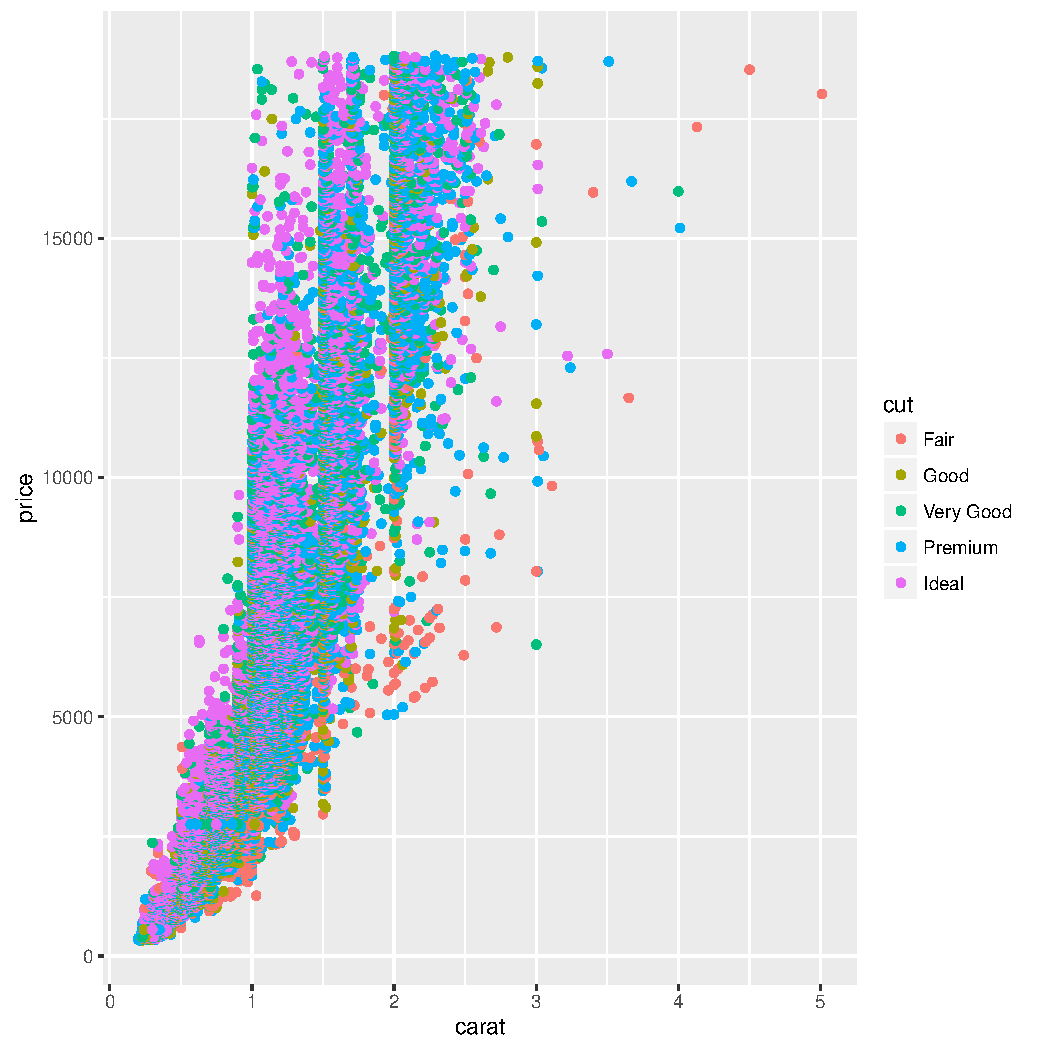
\includegraphics[width=\maxwidth]{figure/unnamed-chunk-1-1} 

\end{knitrout}


Ahora le agregamos al código anterior un tema de ggplot2:\\


$<< >>=$\\
$library('ggplot2') $\\
$qplot(carat, price, data = diamonds, color = cut) +$\\
$theme(legend.text = element_text(size = 12, angle = 45)) +$\\
$theme(legend.position = "bottom")$\\
$@$\\
Con lo que obtenemos \\

\begin{knitrout}
\definecolor{shadecolor}{rgb}{0.969, 0.969, 0.969}\color{fgcolor}\begin{kframe}
\begin{alltt}
\hlkwd{library}\hlstd{(}\hlstr{'ggplot2'}\hlstd{)}
\hlkwd{qplot}\hlstd{(carat, price,} \hlkwc{data} \hlstd{= diamonds,} \hlkwc{color} \hlstd{= cut)} \hlopt{+}
\hlkwd{theme}\hlstd{(}\hlkwc{legend.text} \hlstd{=} \hlkwd{element_text}\hlstd{(}\hlkwc{size} \hlstd{=} \hlnum{12}\hlstd{,} \hlkwc{angle} \hlstd{=} \hlnum{45}\hlstd{))} \hlopt{+}
\hlkwd{theme}\hlstd{(}\hlkwc{legend.position} \hlstd{=} \hlstr{"bottom"}\hlstd{)}
\end{alltt}
\end{kframe}
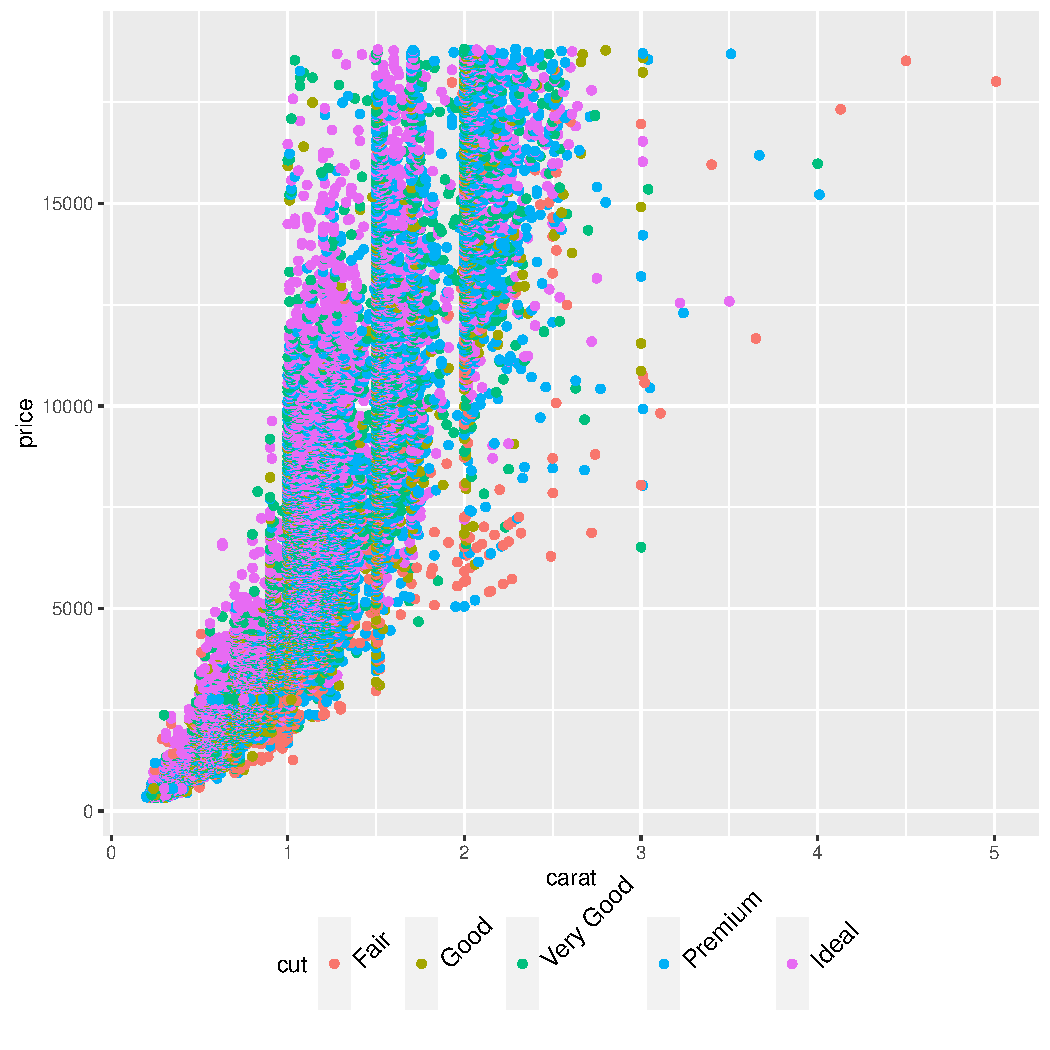
\includegraphics[width=\maxwidth]{figure/unnamed-chunk-2-1} 

\end{knitrout}
Se observa que la segunda grafica cambia con respecto a la primera, si se requiere que todas la graficas tengan el mismo tema se podría copiar el segmento de código que define el tema en todas la graficas pero en caso de querer cambiar alguna característica del tema sería necesario cambiar este parámetro en todas las gráficas con la ayuda de referencias cruzadas esto no es necesario. Para poder simplificar dicha tarea procedemos a darle un nombre o etiqueta a un segmento de código que contenga las características de la gráfica: \\

$<<temagraficas1, eval=FALSE>>=$\\
$theme(legend.text = element_text(size = 12, angle = 45)) +$\\
$theme(legend.position = "bottom")$\\
$@$\\

Ahora podemos realizar nuestra grafica de la siguiente manera:\\

$<<>>=$\\
$qplot(carat, price, data = diamonds, color = cut) +$\\
$<<temagraficas1>>$\\
$@$\\

Como se observa de esta forma R llama el segmento de código con la etiqueta <<temagraficas1>> y ejecuta todos los comandos que contiene dicho segmento.\\


\begin{enumerate}
  \item  \textbf{referencias por segmentos}\\
  Como se mencionó anteriormente es posible utilizar segmentos de códigos a través del documento las veces que se requiera por medio de etiquetas.
  \begin{enumerate}
  \item referencias por segmentos embebidas\\
  Es posible llamar segmentos de códigos dentro de otros segmentos de código por medio de etiquetas, en el siguiente ejemplo utilizaremos la función runif la cual es una distribución uniforme es equiprobable para todos los valores incluidos en un intervalo dado:
$<<A>>=$\\
$x <- runif(1,0,10) $\\
$@$\\
$<<B>>=$\\
$x$\\
$<<A>>$\\
$x$\\
$@$\\
Con lo que obtenemos:

\begin{knitrout}
\definecolor{shadecolor}{rgb}{0.969, 0.969, 0.969}\color{fgcolor}\begin{kframe}
\begin{alltt}
\hlstd{x} \hlkwb{<-} \hlkwd{runif}\hlstd{(}\hlnum{1}\hlstd{,}\hlnum{0}\hlstd{,}\hlnum{10}\hlstd{)}
\end{alltt}
\end{kframe}
\end{knitrout}
\begin{knitrout}
\definecolor{shadecolor}{rgb}{0.969, 0.969, 0.969}\color{fgcolor}\begin{kframe}
\begin{alltt}
\hlstd{x}
\end{alltt}
\begin{verbatim}
## [1] 0.9779362
\end{verbatim}
\begin{alltt}
\hlstd{x} \hlkwb{<-} \hlkwd{runif}\hlstd{(}\hlnum{1}\hlstd{,}\hlnum{0}\hlstd{,}\hlnum{10}\hlstd{)}
\hlstd{x}
\end{alltt}
\begin{verbatim}
## [1] 6.574535
\end{verbatim}
\end{kframe}
\end{knitrout}

Nos damos cuenta que al llamar el segmento A en el segmento B, es como si se copiara todo el contenido de A donde se encuentra la etiqueta $<<A>>$

\item reutilización de todo un segmento de código\\
      En el caso de querer utilizar todo un segmento de código existen dos posibilidades:\\ \\
      1) Usar la misma etiqueta dejándola vacía. \\ \\
$<<chunkA, eval=FALSE>>=$\\
$x <- 5*6$\\
$@$\\
$<<chunkA, eval=TRUE>>=$\\
$@$\\
Lo que da como resultado:\\
\begin{knitrout}
\definecolor{shadecolor}{rgb}{0.969, 0.969, 0.969}\color{fgcolor}\begin{kframe}
\begin{alltt}
\hlstd{x} \hlkwb{<-} \hlnum{5}\hlopt{*}\hlnum{6}
\end{alltt}
\end{kframe}
\end{knitrout}
\begin{knitrout}
\definecolor{shadecolor}{rgb}{0.969, 0.969, 0.969}\color{fgcolor}\begin{kframe}
\begin{alltt}
\hlstd{x} \hlkwb{<-} \hlnum{5}\hlopt{*}\hlnum{6}
\end{alltt}
\end{kframe}
\end{knitrout}
El inconveniente con este código consiste en que no se pueden almacenar los dos segmentos en cache, en el ejemplo anterior el parámetro eval hace referencias que la segunda vez que utilizamos el segmento de código tiene en cuenta el resultado anterior del mismo. \\ \\
 2)	Con la opción ref.label, la cual se utiliza en este caso para unir dos trozos de códigos diferentes en este caso generamos con código C apartir del os códigos A y B: \\ \\
$<<A>>=$\\
$x <- rnorm(1)$\\
$@$\\
$<<B>>=$\\
$y <- x + 2$\\
$@$\\
$<<C, ref.label=c('A', 'B')>>=$\\
$@$\\
Lo que da como resultado:\\
codigo A1
\begin{knitrout}
\definecolor{shadecolor}{rgb}{0.969, 0.969, 0.969}\color{fgcolor}\begin{kframe}
\begin{alltt}
\hlstd{x} \hlkwb{<-} \hlkwd{rnorm}\hlstd{(}\hlnum{1}\hlstd{)}
\end{alltt}
\end{kframe}
\end{knitrout}
codigo B1
\begin{knitrout}
\definecolor{shadecolor}{rgb}{0.969, 0.969, 0.969}\color{fgcolor}\begin{kframe}
\begin{alltt}
\hlstd{y} \hlkwb{<-} \hlstd{x} \hlopt{+} \hlnum{2}
\end{alltt}
\end{kframe}
\end{knitrout}
codigo C
\begin{knitrout}
\definecolor{shadecolor}{rgb}{0.969, 0.969, 0.969}\color{fgcolor}\begin{kframe}
\begin{alltt}
\hlstd{x} \hlkwb{<-} \hlkwd{rnorm}\hlstd{(}\hlnum{1}\hlstd{)}
\hlstd{y} \hlkwb{<-} \hlstd{x} \hlopt{+} \hlnum{2}
\end{alltt}
\end{kframe}
\end{knitrout}

      
\end{enumerate}
\item \textbf{Exteriorización de código} \\

Para obtener un documento mucho más ordenado y estructurado es mejor tener los segmentos de código de R en documentos aporte para esta tarea knitr por medio del script $read\_chunk()$ es posible. Este script se puede utilizar de dos formas usando etiquetas en el guion para separar los segmentos de código o especificar que código ejecutar tomando el número de la línea.
\begin{enumerate}
  \item segmentos por etiqueta \\
  Los comandos de R también utilizan etiquetas de la forma  $\#\#----nombre----$ , es importante denotar que todos los documentos con los cuales se van a trabajar en el documento principal tiene que estar todos en la misma carpeta. se toma como ejemplo el siguiente código de R el cual guardaremos con el nombre de ejemplo1.R\\ \\
  $\#\# ---- D ----$\\
    $m <- 2$\\
    $n <- 5$\\
    $m$\\
    $n$\\ \\ 
    para llamar el código de R en nuestro documento lo primero es ejecutar el script  read\_chunk de la siguiente manera:\\ 

$<<>>=$\\
$read\_chunk("ejemplo1.R")$\\
$@$\\

\begin{knitrout}
\definecolor{shadecolor}{rgb}{0.969, 0.969, 0.969}\color{fgcolor}\begin{kframe}
\begin{alltt}
\hlkwd{read_chunk}\hlstd{(}\hlstr{"ejemplo1.R"}\hlstd{)}
\end{alltt}
\end{kframe}
\end{knitrout}
Posteriormente ya podemos llamar el código por medio de su etiqueta 
$<<D>>=$\\
$@$\\

\begin{knitrout}
\definecolor{shadecolor}{rgb}{0.969, 0.969, 0.969}\color{fgcolor}\begin{kframe}
\begin{alltt}
    \hlstd{m} \hlkwb{<-} \hlnum{2}
    \hlstd{n} \hlkwb{<-} \hlnum{5}
    \hlstd{m}
\end{alltt}
\begin{verbatim}
## [1] 2
\end{verbatim}
\begin{alltt}
    \hlstd{n}
\end{alltt}
\begin{verbatim}
## [1] 5
\end{verbatim}
\end{kframe}
\end{knitrout}
 \item segmentos de códigos basados en líneas \\
 
 $read\_chunk()$ también permite asignar a líneas de código de un archivo de R diferentes etiquetas para ser utilizadas en el documento. Como ejemplo guardamos los numero del 1 al 12 en un archivo con el nombre ejemplo2.R\\
\\1\\2\\4\\5\\6\\7\\8\\9\\10\\12\\ 

Vamos a tomar la línea 1-4,5-8 y 11-12 del archivo de R anterior con ellos formaremos los segmentos de codigo con las etiquetas E, F y G, dicho proceso se realiza de la siguiente manera:\\ 

$read\_chunk("ejemplo2.R", labels = c("E", "F", "G"), from = c(1,5, 11), to = c(4,8,12))$\\ 
\begin{knitrout}
\definecolor{shadecolor}{rgb}{0.969, 0.969, 0.969}\color{fgcolor}\begin{kframe}
\begin{alltt}
\hlkwd{read_chunk}\hlstd{(}\hlstr{"ejemplo2.R"}\hlstd{,} \hlkwc{labels} \hlstd{=} \hlkwd{c}\hlstd{(}\hlstr{"E"}\hlstd{,} \hlstr{"F"}\hlstd{,} \hlstr{"G"}\hlstd{),} \hlkwc{from} \hlstd{=} \hlkwd{c}\hlstd{(}\hlnum{1}\hlstd{,}\hlnum{5}\hlstd{,} \hlnum{11}\hlstd{),} \hlkwc{to} \hlstd{=} \hlkwd{c}\hlstd{(}\hlnum{4}\hlstd{,}\hlnum{8}\hlstd{,}\hlnum{12}\hlstd{))}
\end{alltt}
\end{kframe}
\end{knitrout}


asi podemos llamar cualquiera de los tres segmentos de código en cualquier momento:\\ 

$<<E>>=$\\
$@$\\
$<<F>>=$\\
$@$\\
$<<G>>=$\\
$@$\\
para E:
\begin{knitrout}
\definecolor{shadecolor}{rgb}{0.969, 0.969, 0.969}\color{fgcolor}\begin{kframe}
\begin{alltt}
\hlnum{1}
\end{alltt}
\begin{verbatim}
## [1] 1
\end{verbatim}
\begin{alltt}
\hlnum{2}
\end{alltt}
\begin{verbatim}
## [1] 2
\end{verbatim}
\begin{alltt}
\hlnum{3}
\end{alltt}
\begin{verbatim}
## [1] 3
\end{verbatim}
\begin{alltt}
\hlnum{4}
\end{alltt}
\begin{verbatim}
## [1] 4
\end{verbatim}
\end{kframe}
\end{knitrout}
para F:
\begin{knitrout}
\definecolor{shadecolor}{rgb}{0.969, 0.969, 0.969}\color{fgcolor}\begin{kframe}
\begin{alltt}
\hlnum{5}
\end{alltt}
\begin{verbatim}
## [1] 5
\end{verbatim}
\begin{alltt}
\hlnum{6}
\end{alltt}
\begin{verbatim}
## [1] 6
\end{verbatim}
\begin{alltt}
\hlnum{7}
\end{alltt}
\begin{verbatim}
## [1] 7
\end{verbatim}
\begin{alltt}
\hlnum{8}
\end{alltt}
\begin{verbatim}
## [1] 8
\end{verbatim}
\end{kframe}
\end{knitrout}
para G:
\begin{knitrout}
\definecolor{shadecolor}{rgb}{0.969, 0.969, 0.969}\color{fgcolor}\begin{kframe}
\begin{alltt}
\hlnum{11}
\end{alltt}
\begin{verbatim}
## [1] 11
\end{verbatim}
\begin{alltt}
\hlnum{12}
\end{alltt}
\begin{verbatim}
## [1] 12
\end{verbatim}
\end{kframe}
\end{knitrout}

\end{enumerate}

 \item \textbf{Documentos hijos} \\
 
 De Forma equivalente que se realiza en latex donde se puede tener un archivo principal y muchos documentos hijos que son llamados y compilados por el archivo principal, \textbf{knitr} permite este mismo tratamiento.\\
 
 \begin{enumerate}
  \item entradas de documentos hijos \\
   Como ejemplo se toma como documento principal este mismo documento llamado referenciascruzadas.Rnw y como documento hijo crearemos un documento llamado cap1.Rnw con el siguiente código: \\ \\
   
$<<H1>>=$\\
$y <- sum(x^2)$\\
$@$\\

incluimos el documento hijo de la siguiente forma:

$<<H, child='cap1.Rnw'>>=$\\
$@$\\


\begin{knitrout}
\definecolor{shadecolor}{rgb}{0.969, 0.969, 0.969}\color{fgcolor}\begin{kframe}
\begin{alltt}
\hlstd{y} \hlkwb{<-} \hlkwd{sum}\hlstd{(x}\hlopt{^}\hlnum{2}\hlstd{)}
\end{alltt}
\end{kframe}
\end{knitrout}

Como se observa anteriormente el documento hijo utiliza una variable x para ello llamamos el segmento de codigo <<A>> que genera un numero aleatorio.\\
\begin{knitrout}
\definecolor{shadecolor}{rgb}{0.969, 0.969, 0.969}\color{fgcolor}\begin{kframe}
\begin{alltt}
\hlstd{x} \hlkwb{<-} \hlkwd{runif}\hlstd{(}\hlnum{1}\hlstd{,}\hlnum{0}\hlstd{,}\hlnum{10}\hlstd{)}
\end{alltt}
\end{kframe}
\end{knitrout}
Y si llamamos a H la cual utiliza la variable x, y da como resultado la variable y obtenemos como respuesta de y=1.668906


Cabe denotar que antes de llamar el segmento de codigo H ya tenemos la respuesta y esto debido que al momento de incluir el documento hijo este es compildo.\\
\LaTeX
   
  \item modo independiente \\
  
  Cuando se trabaja con \LaTeX los documentos de \LaTeX tiene un encabezado que les indica que tipo de documento es los paquetes que utiliza entre otras características generales que va tener el documento. Los documentos hijos y códigos de R que se trabajan en Rstudio muchas veces no tiene el encabezado de \LaTeX para poder ser compilados o que son códigos que se generaron de forma ajena al documento pero que queremos adjuntarlos, para estos casos es posible leer y compilar los códigos hijos con el elcabezado del documento principal. \\   \\
  
  La función set\_parent() de knitr aplicada en el documeto hijo toma el encabezado del documento principal de esta forma es posible compilar el codigo hijo sin necesidad de compilar todo el documento principal. Tomando el documento cap1.Rnw si agregamos el siguiente comando al documento hijo: \\

$<<parent, include=FALSE>>=$\\
$set_parent("referenciascruzadas.Rnw ")$\\
$@$\\
Con lo cual el nuevo documento hijo nos quedaría de la siguiente forma: \\ \\ 
$<<parent, include=FALSE>>=$\\
$set_parent("referenciascruzadas.Rnw ")$\\
$@$\\
$<<H1>>=$\\
$y <- sum(x^2)$\\
$@$\\

 Al compilar el documento hijo observamos que compila sin problemas y con las mismas características del documento principal.
  
  
\end{enumerate}

 

\end{enumerate}






\end{document}
